\documentclass[tikz]{standalone}

\usepackage{amsmath}
\usepackage{physics}

\usetikzlibrary{arrows.meta,fit,positioning}

\begin{document}
	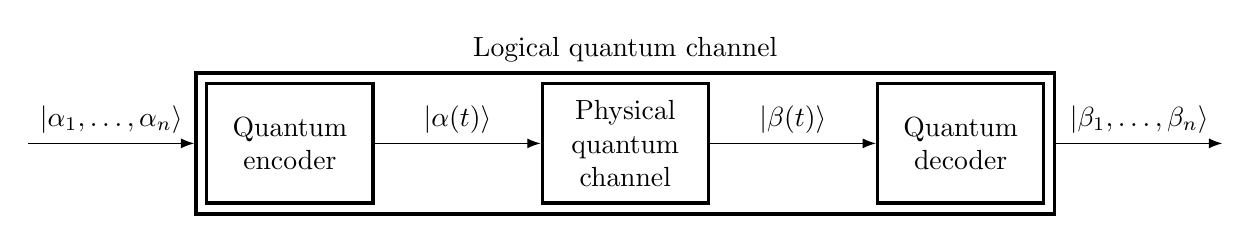
\begin{tikzpicture}[
		node distance=6em,
		block/.style={draw, very thick, minimum height=10ex, minimum width=6em, align=center},
	]
		\node (enc) [block] {Quantum\\encoder};
		\node (pch) [block, right=of enc] {Physical\\quantum\\channel};
		\node (dec) [block, right=of pch] {Quantum\\decoder};
		\node[block, fit=(enc) (dec), label={Logical quantum channel}] (lqc) {};
%		\node[block, below=0.8cm of lqc, minimum height=8ex, minimum width=12em] {Post-processing};
		
		\coordinate[left=6em of lqc] (in);
		\coordinate[right=6em of lqc] (out);
		
		\draw[-Latex] (in) -- node[above]{$\ket{\alpha_1,\dots,\alpha_n}$} (lqc);
		\draw[-Latex] (enc) -- node[above]{$\ket{\alpha(t)}$} (pch);
		\draw[-Latex] (pch) -- node[above]{$\ket{\beta(t)}$} (dec);
		\draw[-Latex] (lqc) -- node[above]{$\ket{\beta_1,\dots,\beta_n}$} (out);
	\end{tikzpicture}
\end{document}
